To relate the calculated attenuation coefficient of a particular object to the effective energy, a $2^\text{nd}$ degree, 4 knot B-spline was used to fit NIST's mass attenuation coefficient data \cite{AttnCoef}, where the mass attenuation coefficient is defined as the attenuation coefficient divided by the object's density, $\mu/\rho$. This fit, implemented with the Python package Scikit-Learn \cite{SKLearn}, provided $\mu = f(E_{\text{eff}})$; however, $E_{\text{eff}} = f(\mu)$ was needed. The described fits are shown in Figure (\ref{figure:NISTSplineFit}).


\begin{figure}[htbp]
    \centering
    \subfigure[Al]{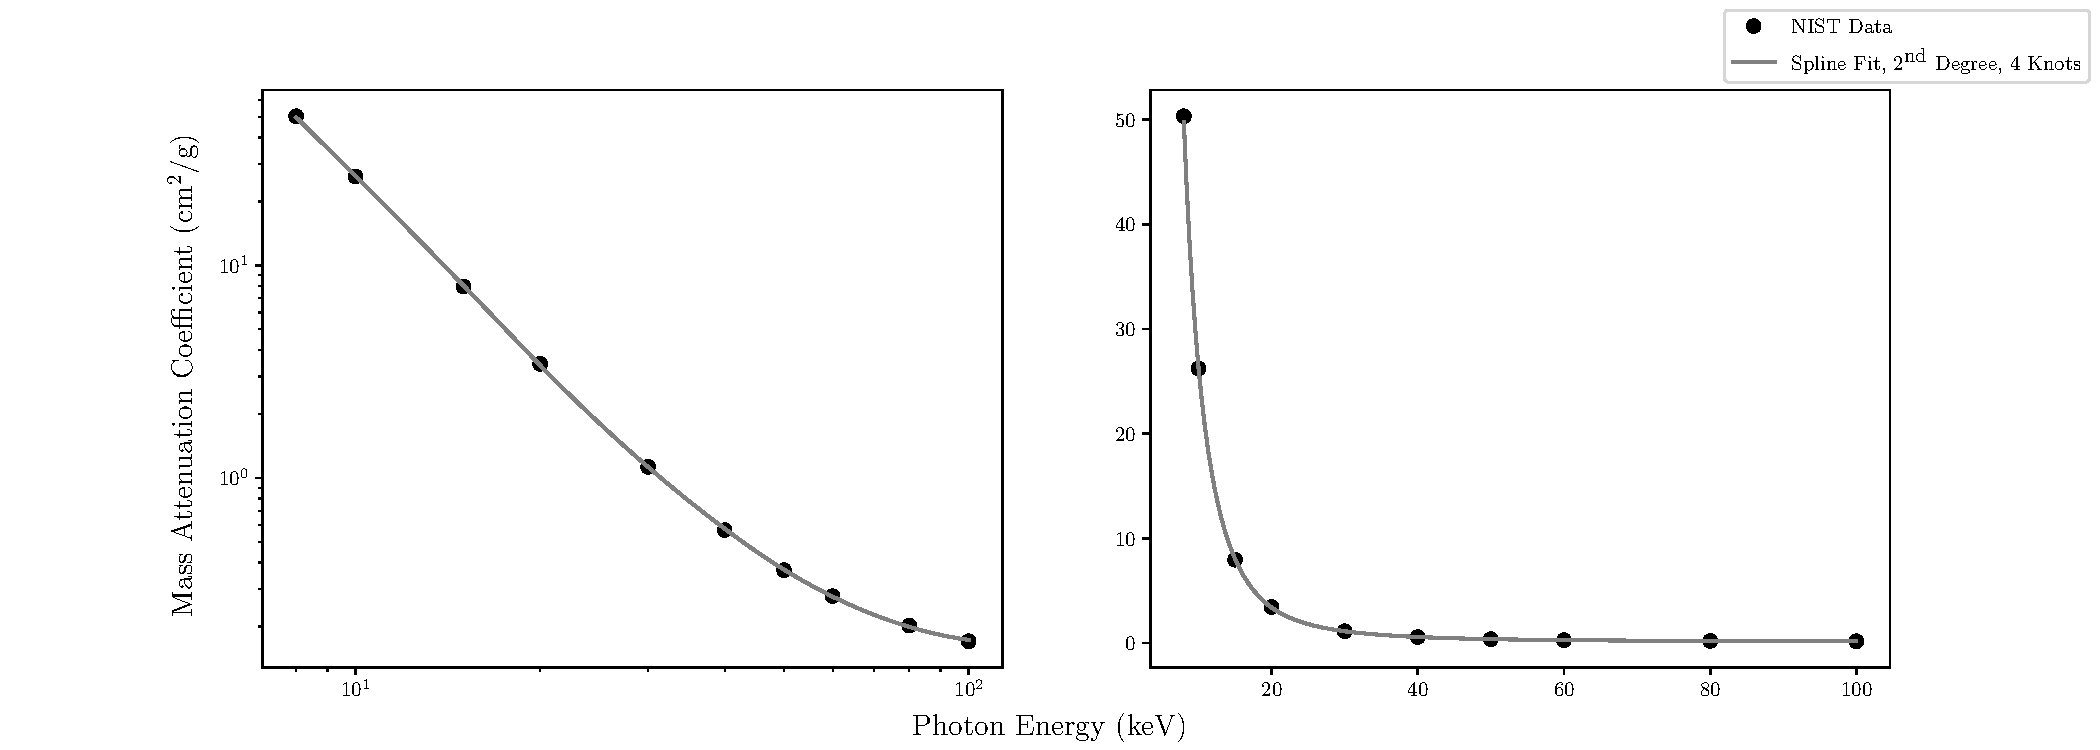
\includegraphics[width=1\linewidth]{Al_NISTSplineFit.pdf}}
    \subfigure[Fe]{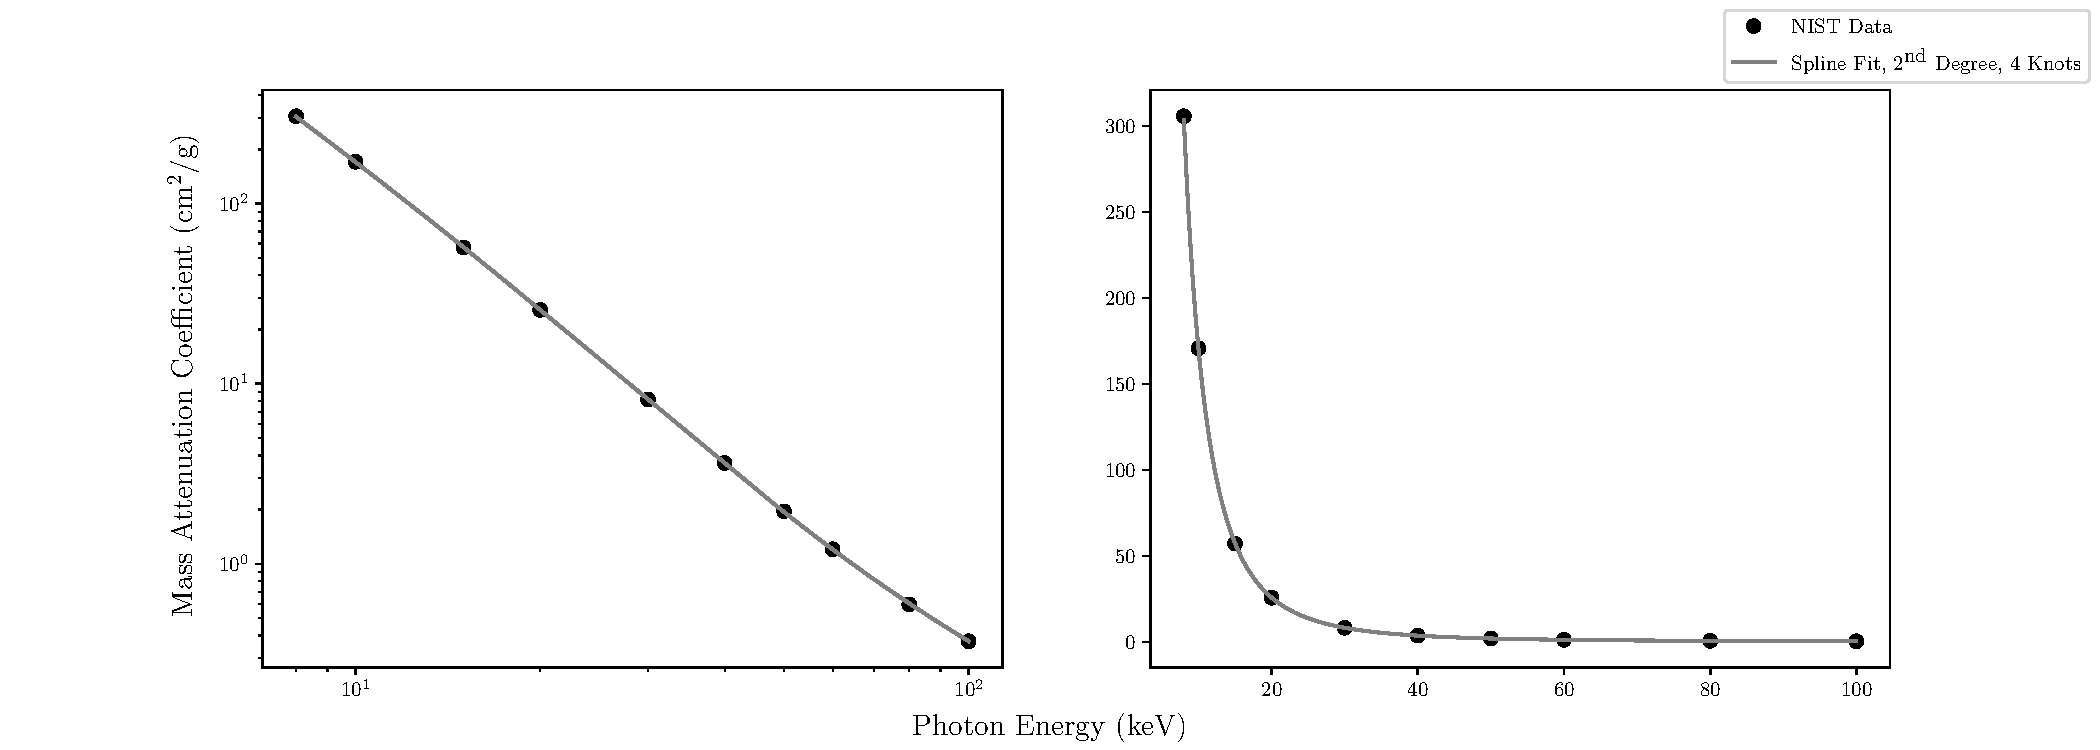
\includegraphics[width=1\linewidth]{Fe_NISTSplineFit.pdf}}
\end{figure}

\begin{figure}[htbp]
    \addtocounter{subfigure}{2}
    \ContinuedFloat
    \addtocounter{figure}{1}
    \centering
    \subfigure[Mg]{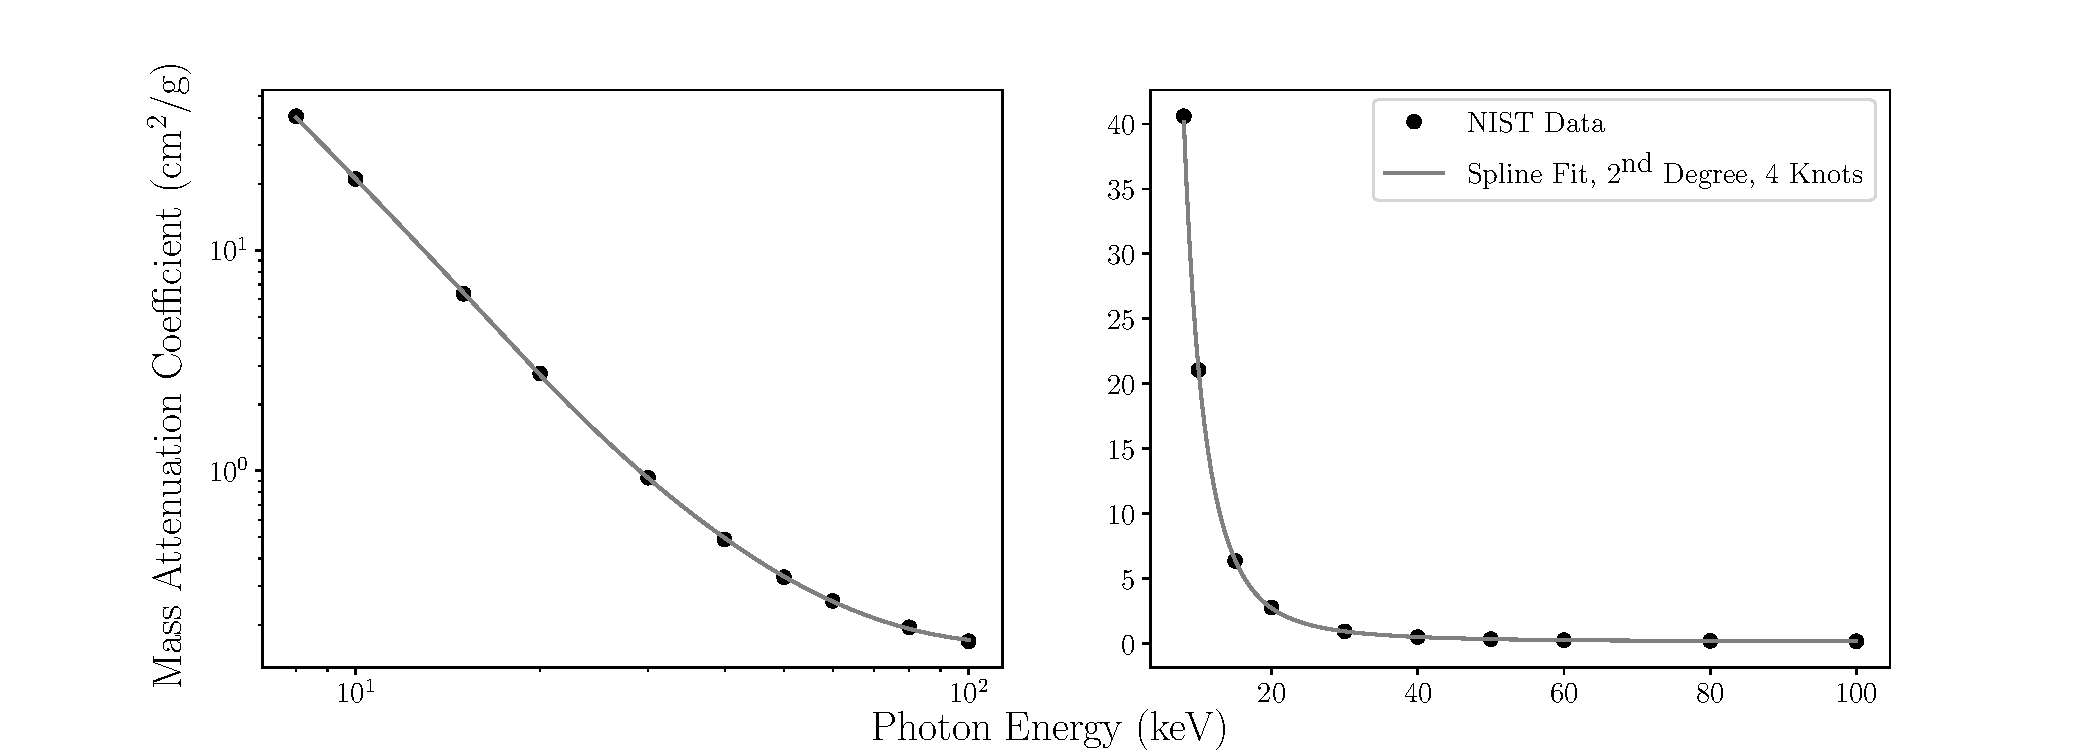
\includegraphics[width=1\linewidth]{Mg_NISTSplineFit.pdf}}
    \subfigure[Plastic Scintillator]{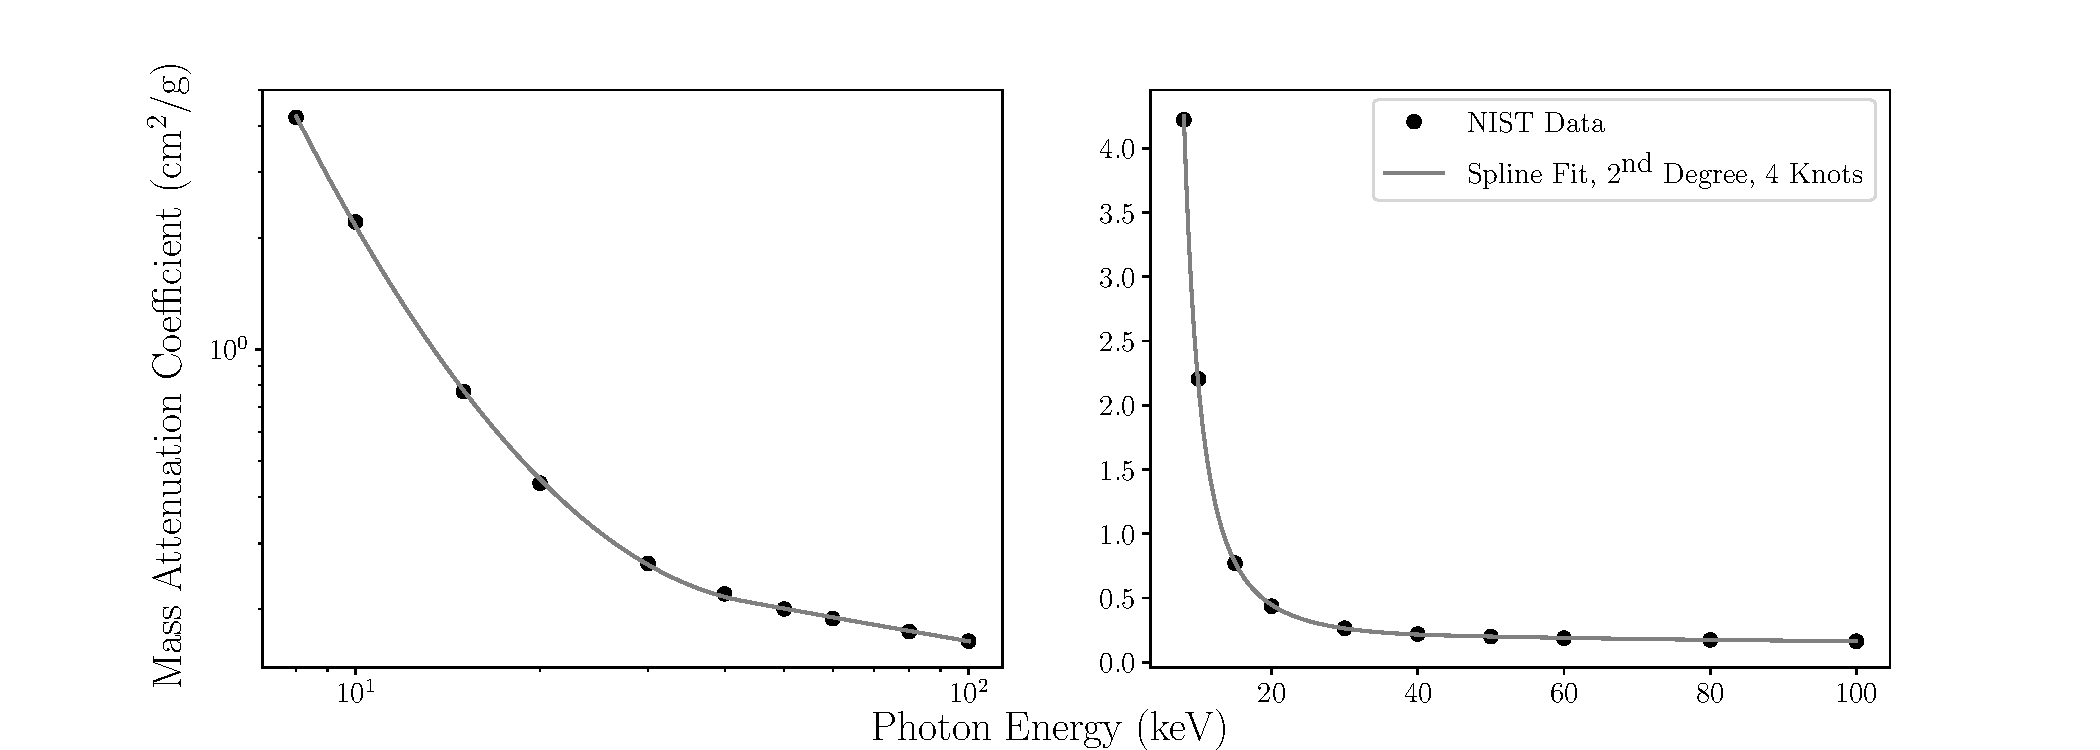
\includegraphics[width=1\linewidth]{Plastic Scintillator (Vinyltoluene-based)_NISTSplineFit.pdf}}
    \subfigure[Water]{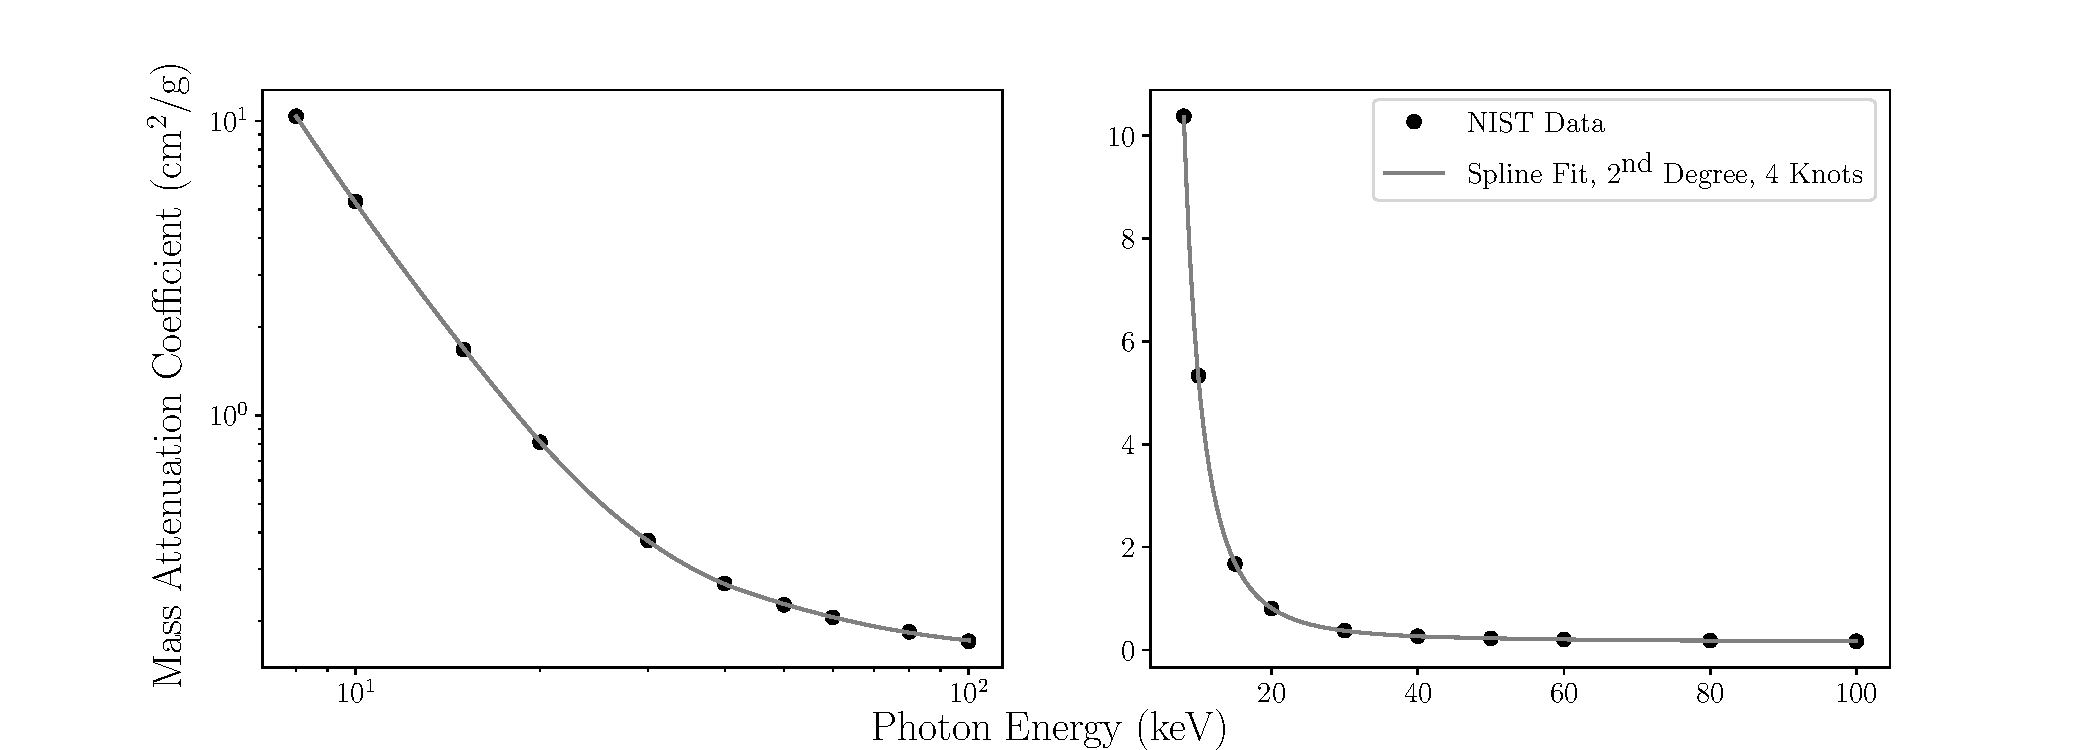
\includegraphics[width=1\linewidth]{Water, Liquid_NISTSplineFit.pdf}}
    \caption{The NIST mass attenuation coefficient data (in cm$^2$/g) vs. effective energy (in keV) for the Al, Fe, Mg, plastic scintillator, and water fitted using the described B-Spline.}
    \label{figure:NISTSplineFit}
\end{figure}

\newpage
Because $f$ represents an abstract model, an inverse was unable to be taken, so an evenly spaced $E_{\text{eff}}$ array of 10,000 values ranging from 0.8 keV to 100 keV was substituted into our model, providing its associated $\mu/\rho$ array. Given a particular $\mu/\rho \pm \sigma$, where $\sigma$ represents the sample standard deviation, Std., of the mass attenuation coefficient, the $E_{\text{eff}}$ was found by first determining the index of the element in the $\mu/\rho$ array closest to the particular $\mu/\rho$. The associated $E_{\text{eff}}$ was then the element in the $E_{\text{eff}}$ array located at the determined index. The range of error for a particular $E_{\text{eff}}$, [$E_{\text{eff}}$ Min, $E_{\text{eff}}$ Max], was calculated by repeating the indexing process for $\mu/\rho + \sigma$ and $\mu/\rho - \sigma$. The results of this indexing technique for each X-ray image can be found in Table (\ref{table::results}).


\begin{table}[H]
    \small
    \noindent\makebox[\textwidth]{%
    \begin{tabularx}{1.27\textwidth}{CCCCCCCCC}

    \toprule
    Material & kVp (kV) &  $I/I_0$ &  $I/I_0$ Std. &  $\mu/\rho$ (cm$^2$/g) &  $\mu/\rho$ Std. (cm$^2$/g) &  $E_{\text{eff}}$ (keV) &  $E_{\text{eff}}$ Max (keV) &  $E_{\text{eff}}$ Min (keV) \\
    \midrule
    & 40.0 &    0.310 &         0.025 &                  1.895 &                       0.131 &                  24.552 &                      25.215 &                      23.954 \\
    & 42.0 &    0.425 &         0.026 &                  1.385 &                       0.099 &                  27.635 &                      28.444 &                      26.917 \\
    Aluminum& 44.0 &    0.567 &         0.025 &                  0.920 &                       0.071 &                  32.576 &                      33.698 &                      31.591 \\
    & 46.0 &    0.668 &         0.023 &                  0.655 &                       0.056 &                  37.747 &                      39.302 &                      36.403 \\
    & 48.0 &    0.727 &         0.023 &                  0.516 &                       0.052 &                  42.145 &                      44.380 &                      40.277 \\
    & 50.0 &    0.888 &         0.020 &                  0.192 &                       0.037 &                  83.926 &                     100.000 &                      69.711 \\
    \midrule
    & 40.0 &    0.353 &         0.030 &                 13.239 &                       1.078 &                  25.316 &                      26.089 &                      24.626 \\
    & 42.0 &    0.432 &         0.031 &                 10.668 &                       0.898 &                  27.331 &                      28.196 &                      26.558 \\
    Iron& 44.0 &    0.595 &         0.030 &                  6.595 &                       0.642 &                  32.392 &                      33.588 &                      31.352 \\
    & 46.0 &    0.678 &         0.027 &                  4.937 &                       0.514 &                  35.870 &                      37.287 &                      34.646 \\
    & 48.0 &    0.761 &         0.028 &                  3.473 &                       0.461 &                  40.599 &                      42.687 &                      38.860 \\
    & 50.0 &    0.911 &         0.024 &                  1.186 &                       0.340 &                  60.335 &                      69.195 &                      54.704 \\
    \midrule
    & 40.0 &    0.632 &         0.030 &                  2.638 &                       0.274 &                  20.200 &                      20.982 &                      19.529 \\
    & 42.0 &    0.832 &         0.029 &                  1.054 &                       0.200 &                  28.444 &                      31.058 &                      26.531 \\
    Magnesium& 44.0 &    0.874 &         0.027 &                  0.776 &                       0.176 &                  32.382 &                      36.412 &                      29.668 \\
    & 46.0 &    0.909 &         0.027 &                  0.551 &                       0.172 &                  37.967 &                      46.193 &                      33.431 \\
    & 48.0 &    0.940 &         0.024 &                  0.353 &                       0.145 &                  48.162 &                      72.627 &                      39.936 \\
    \midrule
    Plastic& 40.0 &    0.578 &          0.03 &                  0.268 &                       0.025 &                  29.392 &                      32.861 &                      27.000 \\
    Scintillator& 42.0 &    0.645 &          0.03 &                  0.215 &                       0.023 &                  40.341 &                      57.906 &                      33.845 \\
    \midrule
    & 44.0 &    0.059 &         0.025 &                  0.489 &                       0.075 &                  25.500 &                      28.076 &                      23.669 \\
    Water & 46.0 &    0.220 &         0.030 &                  0.261 &                       0.024 &                  41.096 &                      46.984 &                      37.369 \\
    & 48.0 &    0.325 &         0.029 &                  0.194 &                       0.015 &                  68.652 &                      86.603 &                      58.403 \\
    \bottomrule
\end{tabularx}
    }
    \caption{The results for each non-saturated (intensities not equal to 0 or 1) X-ray image for the composition experiment.}
    \label{table::results}
\end{table}



The graphs of the $E_{\text{eff}}$ for each kVp and material combination can be found in Figure (\ref{figure::results}). To validate the experimental results, simulated $E_{\text{eff}}$ values were obtained with the Python module SpekPy \cite{SpekPy}, using the X-ray tube assembly specifications as provided by the manufacturer \cite{CArm}.


\begin{figure}[H]
    \centering
    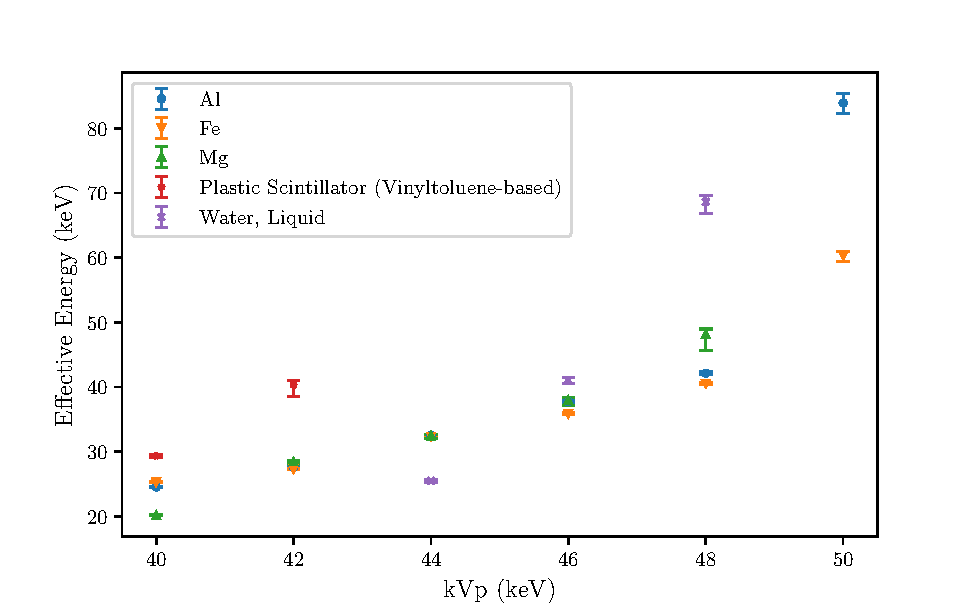
\includegraphics[width=1\linewidth]{effEnergy.pdf}
    \caption{Graph of effective energy (in keV) vs. kVp (in kV) for the X-ray image data contained in Table (\ref{table::results}).}
    \label{figure::results}
\end{figure}

Figure (\ref{figure::results}) shows relative agreement and an approximately linear increase for the Al, Fe, and Mg, up until 50 kVp, where a sudden spike in $E_{\text{eff}}$ is observed. For the plastic scintillator and water, vastly different values are observed. Upon further inspection by increasing the range of the fit shown in Figure (\ref{figure:NISTSplineFit}), the two values increase at an exponential rate. Furthermore, the rate of increase of $E_{\text{eff}}$ with respect to kVp is greater for the monoatomic attenuators in the experiment compared to their simulated values.

For the offset experiment, the intensity values for the image with the centered Al (labeled N) were obtained with the extraction code in the appendix. On the other hand, the intensity values for the image with the offset Al were obtained manually using the software ImageJ. \cite{ImageJ}. The results of this experiment can be found in Table (\ref{table::offset})


\begin{table}[H]
    \small
    \noindent\makebox[\textwidth]{%
    \begin{tabularx}{1.15\textwidth}{cccccccc}
    \toprule
    Position & $I/I_0$ &  $I/I_0$ Std. &  $\mu/\rho$ (cm$^2$/g) &  $\mu/\rho$ Std. (cm$^2$/g) &  $E_{\text{eff}}$ (keV) &  $E_{\text{eff}}$ Max (keV) &  $E_{\text{eff}}$ Min (keV) \\
    \midrule
    Center   &  0.310   &   0.025       &   1.90                &   0.13                        &   24.55                &  25.21                       &   24.00 \\
    Offset   &  0.14    &   0.05        &   3.2                 &   0.5                         &   20.5                 &  21.9                        &   19.4  \\
    \bottomrule
\end{tabularx}               

    }
    \caption{The results of X-ray images of a centered and offset Al (labeled N) at 40 kVp for use in the offset experiment.}
    \label{table::offset}
\end{table}

The results of this experiment show unexpected discrepancies between the centered and offset Al. A slight difference in $E_{\text{eff}}$ is expected due to the point-like nature of the x-ray source; however, it can not explain the statistical nonequivalency observed due to the large distance (44.95 cm)\cite{CArm} between the x-ray source and detector; therefore, demonstrating a dependence on the object's position in the imaging area for the $E_{\text{eff}}$.


For the thickness-varying experiment, x-ray images of Al were taken at 40 kVp. The thickness of the Al was varied by using two different attenuators, one of thickness 2.286 mm (labeled N) and the other of thickness 0.813 mm (labeled I), as found in Table (\ref{table::matTable}). The intensity values for each image were obtained with the code in Code Listing (\ref{code::extractionCode}). The results of this experiment can be found in Table (\ref{table::thickness}).

\begin{table}[H]
    \small
    \noindent\makebox[\textwidth]{%
    \begin{tabularx}{1.2\textwidth}{CCCCCCCC}
    \toprule
    Thickness (mm) & $I/I_0$ &  $I/I_0$ Std. &  $\mu/\rho$ (cm$^2$/g) &  $\mu/\rho$ Std. (cm$^2$/g) &  $E_{\text{eff}}$ (keV) &  $E_{\text{eff}}$ Max (keV) &  $E_{\text{eff}}$ Min (keV) \\
    \midrule
    2.286          & 0.310   &  0.025        &  1.90                  &     0.13                    &   24.55                 &     25.21                   &   24.00   \\
    0.813          & 0.575   &  0.029        &  2.52                  &     0.23                    &   22.15                 &     22.92                   &   21.39   \\
    \bottomrule
\end{tabularx}
    }
    \caption{The results of X-ray images of Al (labeled N) and Al (labeled I) at 40 kVp for use in the thickness-varying experiment.}
   	\label{table::thickness}
\end{table}

The results of this experiment, once again, show unexpected discrepancies in $E_{\text{eff}}$ between the two thicknesses. While the $E_{\text{eff}}$'s are closer than what was measured for the offset experiment, the two values are statistically nonequivalent; therefore, demonstrating a thickness dependence of the $E_{\text{eff}}$.















